\documentclass[a4paper,12pt]{article}
\usepackage[T1]{fontenc}
\usepackage[utf8]{inputenc}
\usepackage[portuguese]{babel}
\usepackage{float}
\usepackage[round]{natbib}
\usepackage[pdftex]{pdfpages}

\usepackage{Sweave}
\begin{document}
\Sconcordance{concordance:DocAula.tex:DocAula.Rnw:%
1 8 1 1 0 4 1 1 6 1 1 1 8 1 1 1 42 19 1 1 2 10 0 1 2 2 1 1 2 35 0 1 2 3 %
1}

% Uso do Comentário
% Para ter chunk CRLT+ALT+I







\title{Análise Descrtiva dos Dados}

\author{Aluno: Matheus Raphael Elero}

\maketitle

\section{Introdução}

Aqui vai um arquivo com os comandos do ''knitr''

Para incluir um pdf, usamos o pacote ''pdfpages''

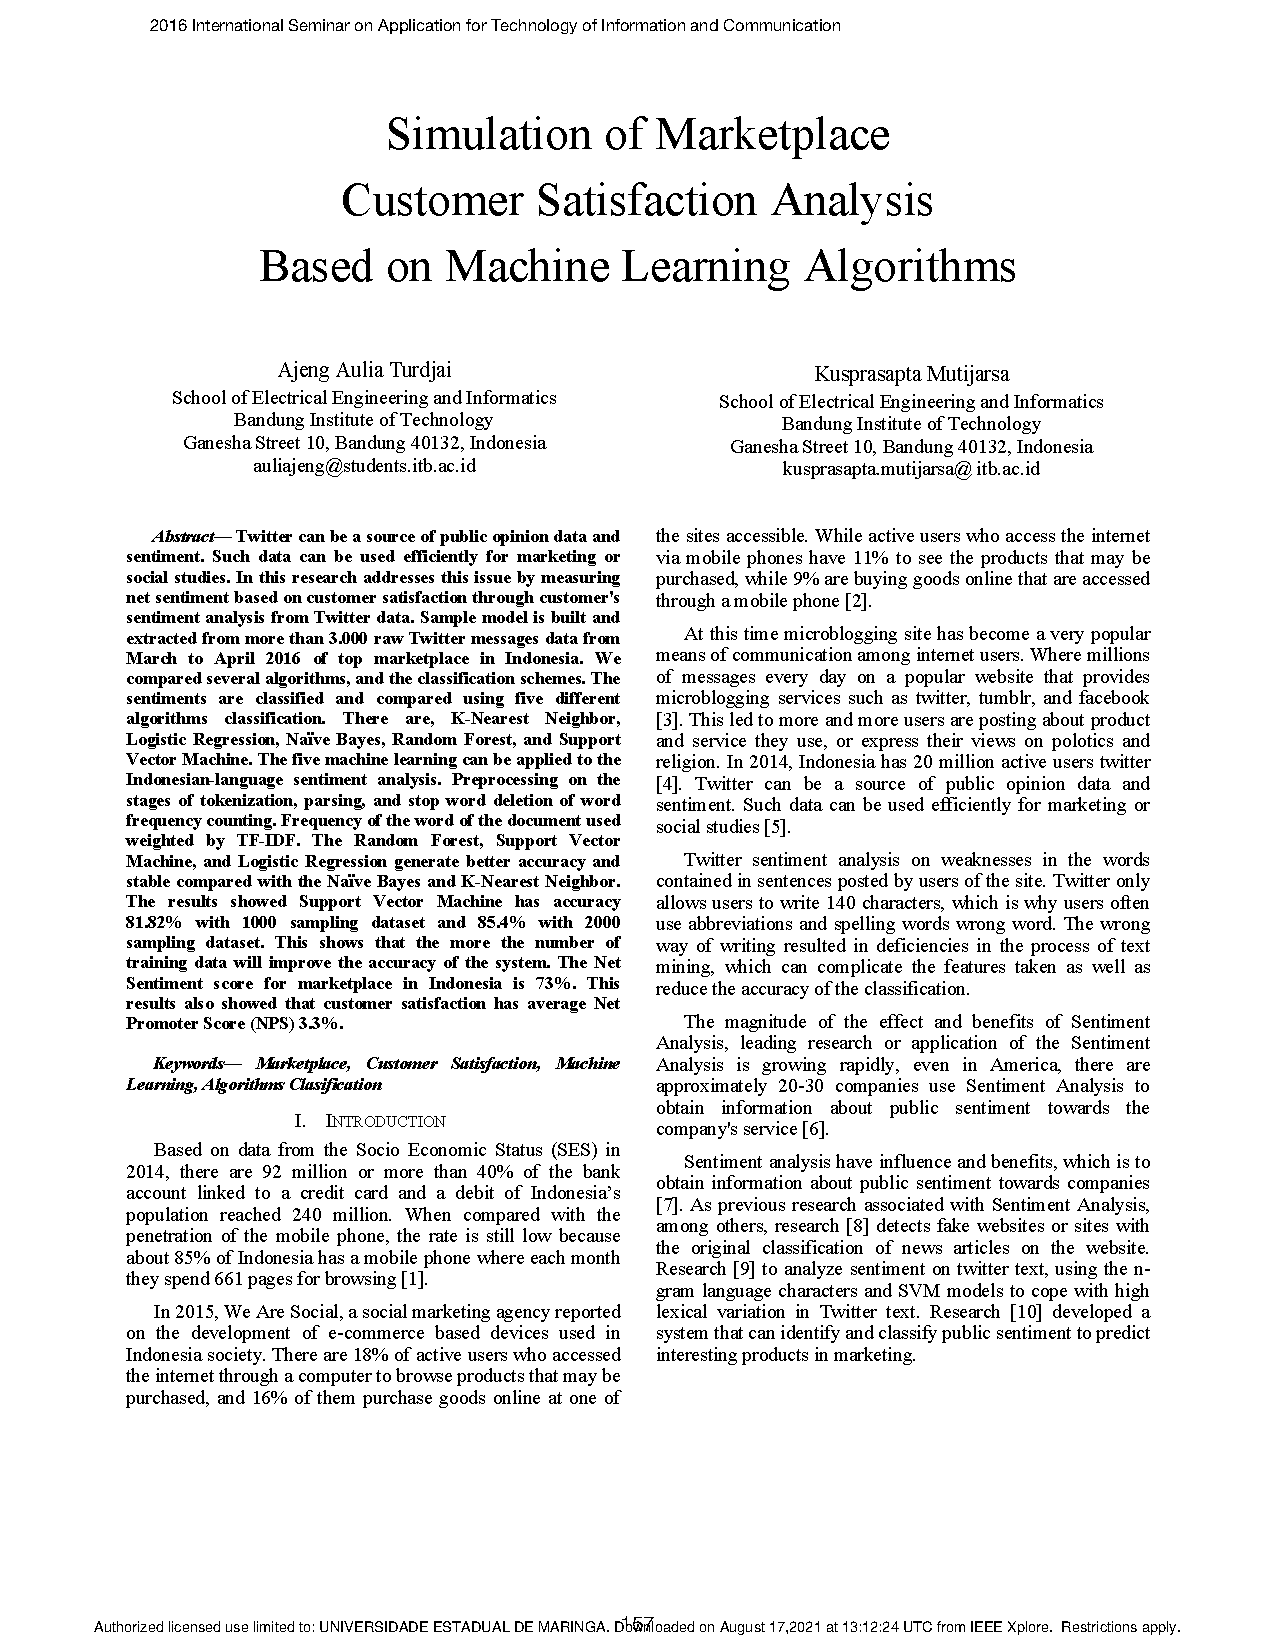
\includepdf[pages=1]{Artigo.pdf}

\section{Dados}

%Arquivo> Contar a história dos dados, escrever o que representa a situação

\begin{Schunk}
\begin{Soutput}
  ind carat     cut color clarity depth table price direcao coord
1   1  0.23   Ideal     E     SI2  61.5    55   326       x  3.95
2   1  0.23   Ideal     E     SI2  61.5    55   326       y  3.98
3   1  0.23   Ideal     E     SI2  61.5    55   326       z  2.43
4   2  0.21 Premium     E     SI1  59.8    61   326       x  3.89
5   2  0.21 Premium     E     SI1  59.8    61   326       y  3.84
6   2  0.21 Premium     E     SI1  59.8    61   326       z  2.31
\end{Soutput}
\end{Schunk}

\section{Tipo de Variáveis}

\begin{Schunk}
\begin{Soutput}
$ind
[1] "integer"

$carat
[1] "numeric"

$cut
[1] "ordered" "factor" 

$color
[1] "ordered" "factor" 

$clarity
[1] "ordered" "factor" 

$depth
[1] "numeric"

$table
[1] "numeric"

$price
[1] "integer"

$x
[1] "numeric"

$y
[1] "numeric"

$z
[1] "numeric"
\end{Soutput}
\end{Schunk}



\end{document}
